%%%%%%%%%%%%%%%%%%%%%%%%% NOTE %%%%%%%%%%%%%%%%%%%%%%%%%%%%
%% You can ignore everything from here until             %%
%% "Question 1: Introduction"                            %%
%%%%%%%%%%%%%%%%%%%%%%%%%%%%%%%%%%%%%%%%%%%%%%%%%%%%%%%%%%%
\documentclass[8pt]{article}
\usepackage{amsmath, amsfonts, amsthm, amssymb}  % Some math symbols
\usepackage{fullpage}
\usepackage{graphicx}
\usepackage[x11names, rgb]{xcolor}
\usepackage{graphicx}
\usepackage{tikz}
\usetikzlibrary{decorations,arrows,shapes}
\usepackage{float} % Add this package to control float placement
\usepackage{etoolbox}
\usepackage{enumerate}
\usepackage{listings}
\usepackage{multicol}
\usepackage{enumitem}
\setlist{nolistsep}
\lstset{
    language=Python,           % Set the language of the code
    basicstyle=\footnotesize\ttfamily,
    keywordstyle=\color{blue}, % Set color for keywords
    commentstyle=\color{gray}, % Set color for comments
    stringstyle=\color{red},   % Set color for strings
    numbers=left,              % Display line numbers on the left
    numberstyle=\tiny\color{gray}, % Style for line numbers
    frame=single,              % Add a frame around the code
    breaklines=true            % Allow line breaking
}


\setlength{\parindent}{0pt}
\setlength{\parskip}{5pt plus 1pt}

\newcommand{\N}{\mathbb N}
\newcommand{\E}{\mathbb E}
\newcommand{\V}{Var}
\renewcommand{\P}{\mathbb P}
\newcommand{\f}{\frac}


\newcommand{\nopagenumbers}{
    \pagestyle{empty}
}

\def\indented#1{\list{}{}\item[]}
\let\indented=\endlist

\providetoggle{questionnumbers}
\settoggle{questionnumbers}{true}
\newcommand{\noquestionnumbers}{
    \settoggle{questionnumbers}{false}
}

\newcounter{questionCounter}
\newenvironment{question}[2][\arabic{questionCounter}]{%
    \addtocounter{questionCounter}{1}%
    \setcounter{partCounter}{0}%
    \vspace{.25in} \hrule \vspace{0.4em}%
        \noindent{\bf \iftoggle{questionnumbers}{#1: }{}#2}%
    \vspace{0.8em} \hrule \vspace{.10in}%
}{$ $\newpage}

\newcounter{partCounter}[questionCounter]
\renewenvironment{part}[1][\alph{partCounter}]{%
    \addtocounter{partCounter}{1}%
    \vspace{.10in}%
    \begin{indented}%
       {\bf (#1)} %
}{\end{indented}}

\def\show#1{\ifdefempty{#1}{}{#1\\}}

\newcommand{\header}{%
\begin{center}
    {\Large \show\myhwname}
    \show\myname
    \show\myemail
    \show\mysection
    \show\hwname
\end{center}}

\usepackage{hyperref} % for hyperlinks
\hypersetup{
    colorlinks=true,
    linkcolor=blue,
    filecolor=magenta,      
    urlcolor=blue,
}

%%%%%%%%%%%%%%%%% Identifying Information %%%%%%%%%%%%%%%%%
%% For 312, we'd rather you DIDN'T tell us who you are   %%
%% in your homework so that we're not biased when        %%
%% So, even if you fill this information in, it will not %%
%% show up in the document unless you uncomment \header  %%
%% below                                                 %%
%%%%%%%%%%%%%%%%%%%%%%%%%%%%%%%%%%%%%%%%%%%%%%%%%%%%%%%%%%%
\newcommand{\myhwname}{DS284: Numerical Linear Algebra}
\newcommand{\myname}{Naman Pesricha}
\newcommand{\myemail}{namanp@iisc.ac.in}
\newcommand{\hwname}{\textbf{Assignment 4}}
\newcommand{\mysection}{SR - 24115}
%%%%%%%%%%%%%%%%%%%%%%%%%%%%%%%%%%%%%%%%%%%%%%%%%%%%%%%%%%%

%%%%%%%%%%%%%%%%%%% Document Options %%%%%%%%%%%%%%%%%%%%%%
\noquestionnumbers
\nopagenumbers
%%%%%%%%%%%%%%%%%%%%%%%%%%%%%%%%%%%%%%%%%%%%%%%%%%%%%%%%%%%

\begin{document}
\header
\begin{question} {Problem 3 \\
Given the matrix:
\[
A = \begin{pmatrix}
0.70000 & 0.70711 \\
0.70001 & 0.70711
\end{pmatrix}
\]
(a) Consider a computer which rounds all computed results to five digits of relative accuracy. Using either Classical Gram-Schmidt (CGS) or Modified Gram-Schmidt (MGS), compute the matrix $Q$ associated with the QR decomposition of $A$ assuming you are working on such a computer.

(b) Apply Householder’s method to compute the QR factorization of $A$ using the same 5-digit arithmetic. \\ Compare the matrices $Q's$ obtained in (a) and (b), and comment on the orthogonality of the $Q$ matrix.}

\end{question}

\begin{question}{Problem 5 \\
In this problem, you will test different algorithms for the least squares problem to approximate the function \( f(t) = \sin(10t) \) for \( t \in [0,1] \) using a polynomial fit. To this end, first generate \( m = 100 \) data points using the above function, which forms your given data, i.e., \( (t_i, f(t_i)) \) for \( i = 1, \dots, m \). Using this data, we would like to construct a 14th-degree least squares polynomial fit to \( f(t) \). Determine its least squares fit using the following methods:

\begin{enumerate}
    \item[(a)] Use QR Factorization with your implementation of Modified Gram-Schmidt. You should write your own back-substitution code for solving the resulting triangular system.
    
    \item[(b)] Using QR Factorization with your implementation of Householder factorization.
    
    \item[(c)] Using SVD (Computed with any inbuilt libraries in MATLAB/Python/Octave).
    
    \item[(d)] Using normal equations, you can use the backslash command in MATLAB to solve this system.
\end{enumerate}

Accept the MATLAB/Octave/Python least squares solution (given by "backslash" \( \backslash \) in MATLAB) as the truth. Display and plot the approximation given by this "true" solution and compare it with \( f(t) \). Compare with the solutions given by the 4 methods described above. Explain the results.
}

To explain our findings, we will calculate 2-norm relative condition numbers 
describing the sensitivities of y and x to perturbations in b and A.

\begin{center}
    Data : A, b; Solutions = x,y;
    \[
        \begin{array}{c|c|c}
          & y & x \\
        \hline
        b & \frac{1}{\cos\theta} & \frac{\kappa(A)}{\eta\cos\theta} \\
        \hline
        A & \frac{\kappa(A)}{\cos\theta} & \kappa(A) + \frac{\kappa(A)^2 \tan\theta}{\eta}
        \end{array}
        \quad = \quad
        \begin{array}{c|c|c}
          & y & x \\
        \hline
        b & 1.000000 \times 10^{0} & 6.187516 \times 10^{3} \\
        \hline
        A & 3.016178 \times 10^{8} & 3.036732 \times 10^{8} \\
        \end{array}
    \]

\end{center}


\textbf{Notation:} In our problem , $b \equiv f$, $x \equiv c$ and for a specific algorithm. The problem we want to solve is \fbox{$Ax = b \equiv Ac = f$}. For a specific algo, the predicted outputs are represented by $f_{algo},\ c_{algo}$ which represents the predicted value $f_{pred}$ and predicted coefficients of polynomial $c_{algo}$ for the algo.

We will write the methodologies used for each computation. \\
\hrule
\begin{multicols}{2}

\begin{enumerate}
    \item \fbox{\textbf{QR using Modified Gram-Schmidt}}
    \begin{align*}
        &Ac = f \\
        &QRc = f \\
        &Rc = Q^{T}f \\
        &\text{Use back-substitution.}
    \end{align*}

    \item \fbox{\textbf{QR using Householder}}
    \begin{align*}
        &\text{Compute Householder to get } R \text{ and } Q^{T}f \\
        &Rc = Q^{T}f \\
        &\text{Use back-substitution to get } c.
    \end{align*}
\end{enumerate}

\columnbreak

\begin{enumerate}
    \setcounter{enumi}{2}
    \item \fbox{\textbf{SVD using $np.linalg.svd$}}
    \begin{align*}
        &\text{Compute SVD.} \\
        &\text{Compute } \hat{U^{T}}b. \\
        &\text{Solve for } \tilde{w} \text{ in } \hat{\Sigma} \tilde{w} = \hat{U^{T}} b. \\
        &\text{Solve for } x \text{ in } V^T x = \tilde{w}.
    \end{align*}

    \item \fbox{\textbf{Normal Equations (MATLAB \textbackslash)}}
    \begin{align*}
        &A^T A x = A^T b \\
        &\text{In MATLAB, use the $\backslash$ command.} 
    \end{align*}
\end{enumerate}

\end{multicols}

\hrule

True solutions are obtained by using MATLAB $\backslash$ command for the equation \fbox{$Ac = f$}. \\

We will now plot the outputs for each of the methods. Note machine epsilon for the computer used is \fbox{$\epsilon_{m} \approx 2.22 \times 10 ^ {-16}$}
\begin{figure}[H]
    \centering
    \begin{subfigure}[b]{0.8\textwidth}
        \centering
        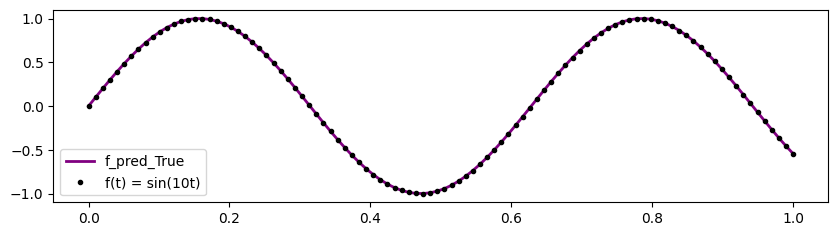
\includegraphics[width=\textwidth]{images/true.png}
        \caption{Caption for Image 1}
        \label{fig:image1}
    \end{subfigure}

    \begin{subfigure}[b]{0.8\textwidth}
        \centering
        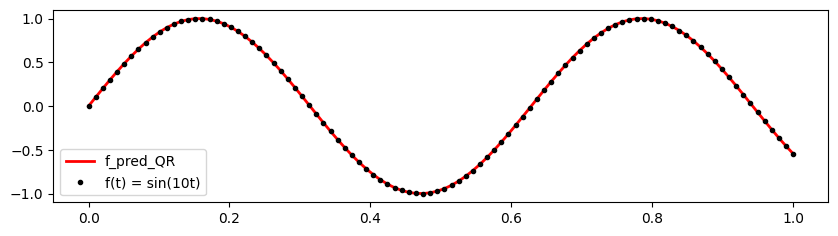
\includegraphics[width=\textwidth]{MGS.png}
        \caption{Caption for Image 2}
        \label{fig:image2}
    \end{subfigure}

    \begin{subfigure}[b]{0.8\textwidth}
        \centering
        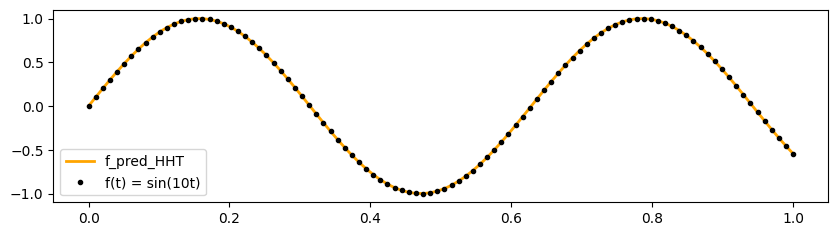
\includegraphics[width=\textwidth]{HHT.png}
        \caption{Caption for Image 3}
        \label{fig:image3}
    \end{subfigure}

    \begin{subfigure}[b]{0.8\textwidth}
        \centering
        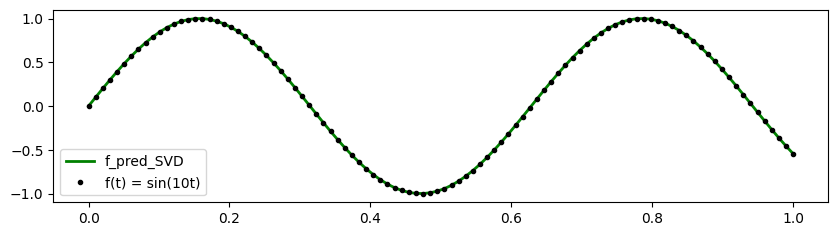
\includegraphics[width=\textwidth]{SVD.png}
        \caption{Caption for Image 4}
        \label{fig:image4}
    \end{subfigure}

    \begin{subfigure}[b]{0.8\textwidth}
        \centering
        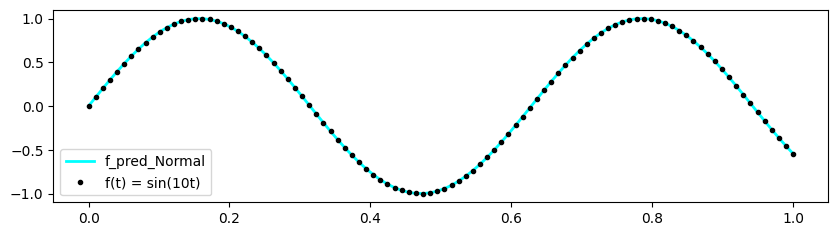
\includegraphics[width=\textwidth]{normal.png}
        \caption{Caption for Image 5}
        \label{fig:image5}
    \end{subfigure}

    \caption{Collection of Images}
    \label{fig:collection}
\end{figure}

\end{question}



\end{document}


